\section{EXPERIMENTS}

\subsection{Experimental Setup}

\subsubsection{Datasets and Tasks}
\begin{itemize}
    \item \textbf{NLU benchmarks}:
    \begin{itemize}
        \item SST-2 for sentiment analysis task
        \item QQP for paraphrase detection task  
        \item STS-B semantic similarity task
    \end{itemize}
    \item \textbf{Federated data partitioning strategies}: IID vs non-IID
\end{itemize}

\subsubsection{Baselines}
\begin{itemize}
    \item Centralized multi-task training
    \item Federated single-task learning
    \item Large model-based federated approaches
\end{itemize}

\subsubsection{Evaluation Metrics}
\begin{itemize}
    \item \textbf{Task-level metrics}:
    \begin{itemize}
        \item SST-2: sentiment analysis task: accuracy \& F1
        \item QQP: paraphrase detection task: accuracy \& F1
        \item STS-B: semantic similarity task: Pearson correlation \& Spearman correlation
    \end{itemize}
    \item \textbf{Federated metrics}: communication rounds, convergence speed
\end{itemize}

\subsubsection{Implementation Details}
\begin{itemize}
    \item Training configuration, hardware, hyperparameters
    \item Model architectures: distil-bert, medium-bert, mini-bert, mini-lm, tiny\_bert
    \item Total experiments: 50 configurations
\end{itemize}

\subsection{Results}

\subsubsection{Overall Multi-Task Performance}
\begin{figure}[h]
    \centering
    \begin{minipage}{0.45\textwidth}
        \centering
        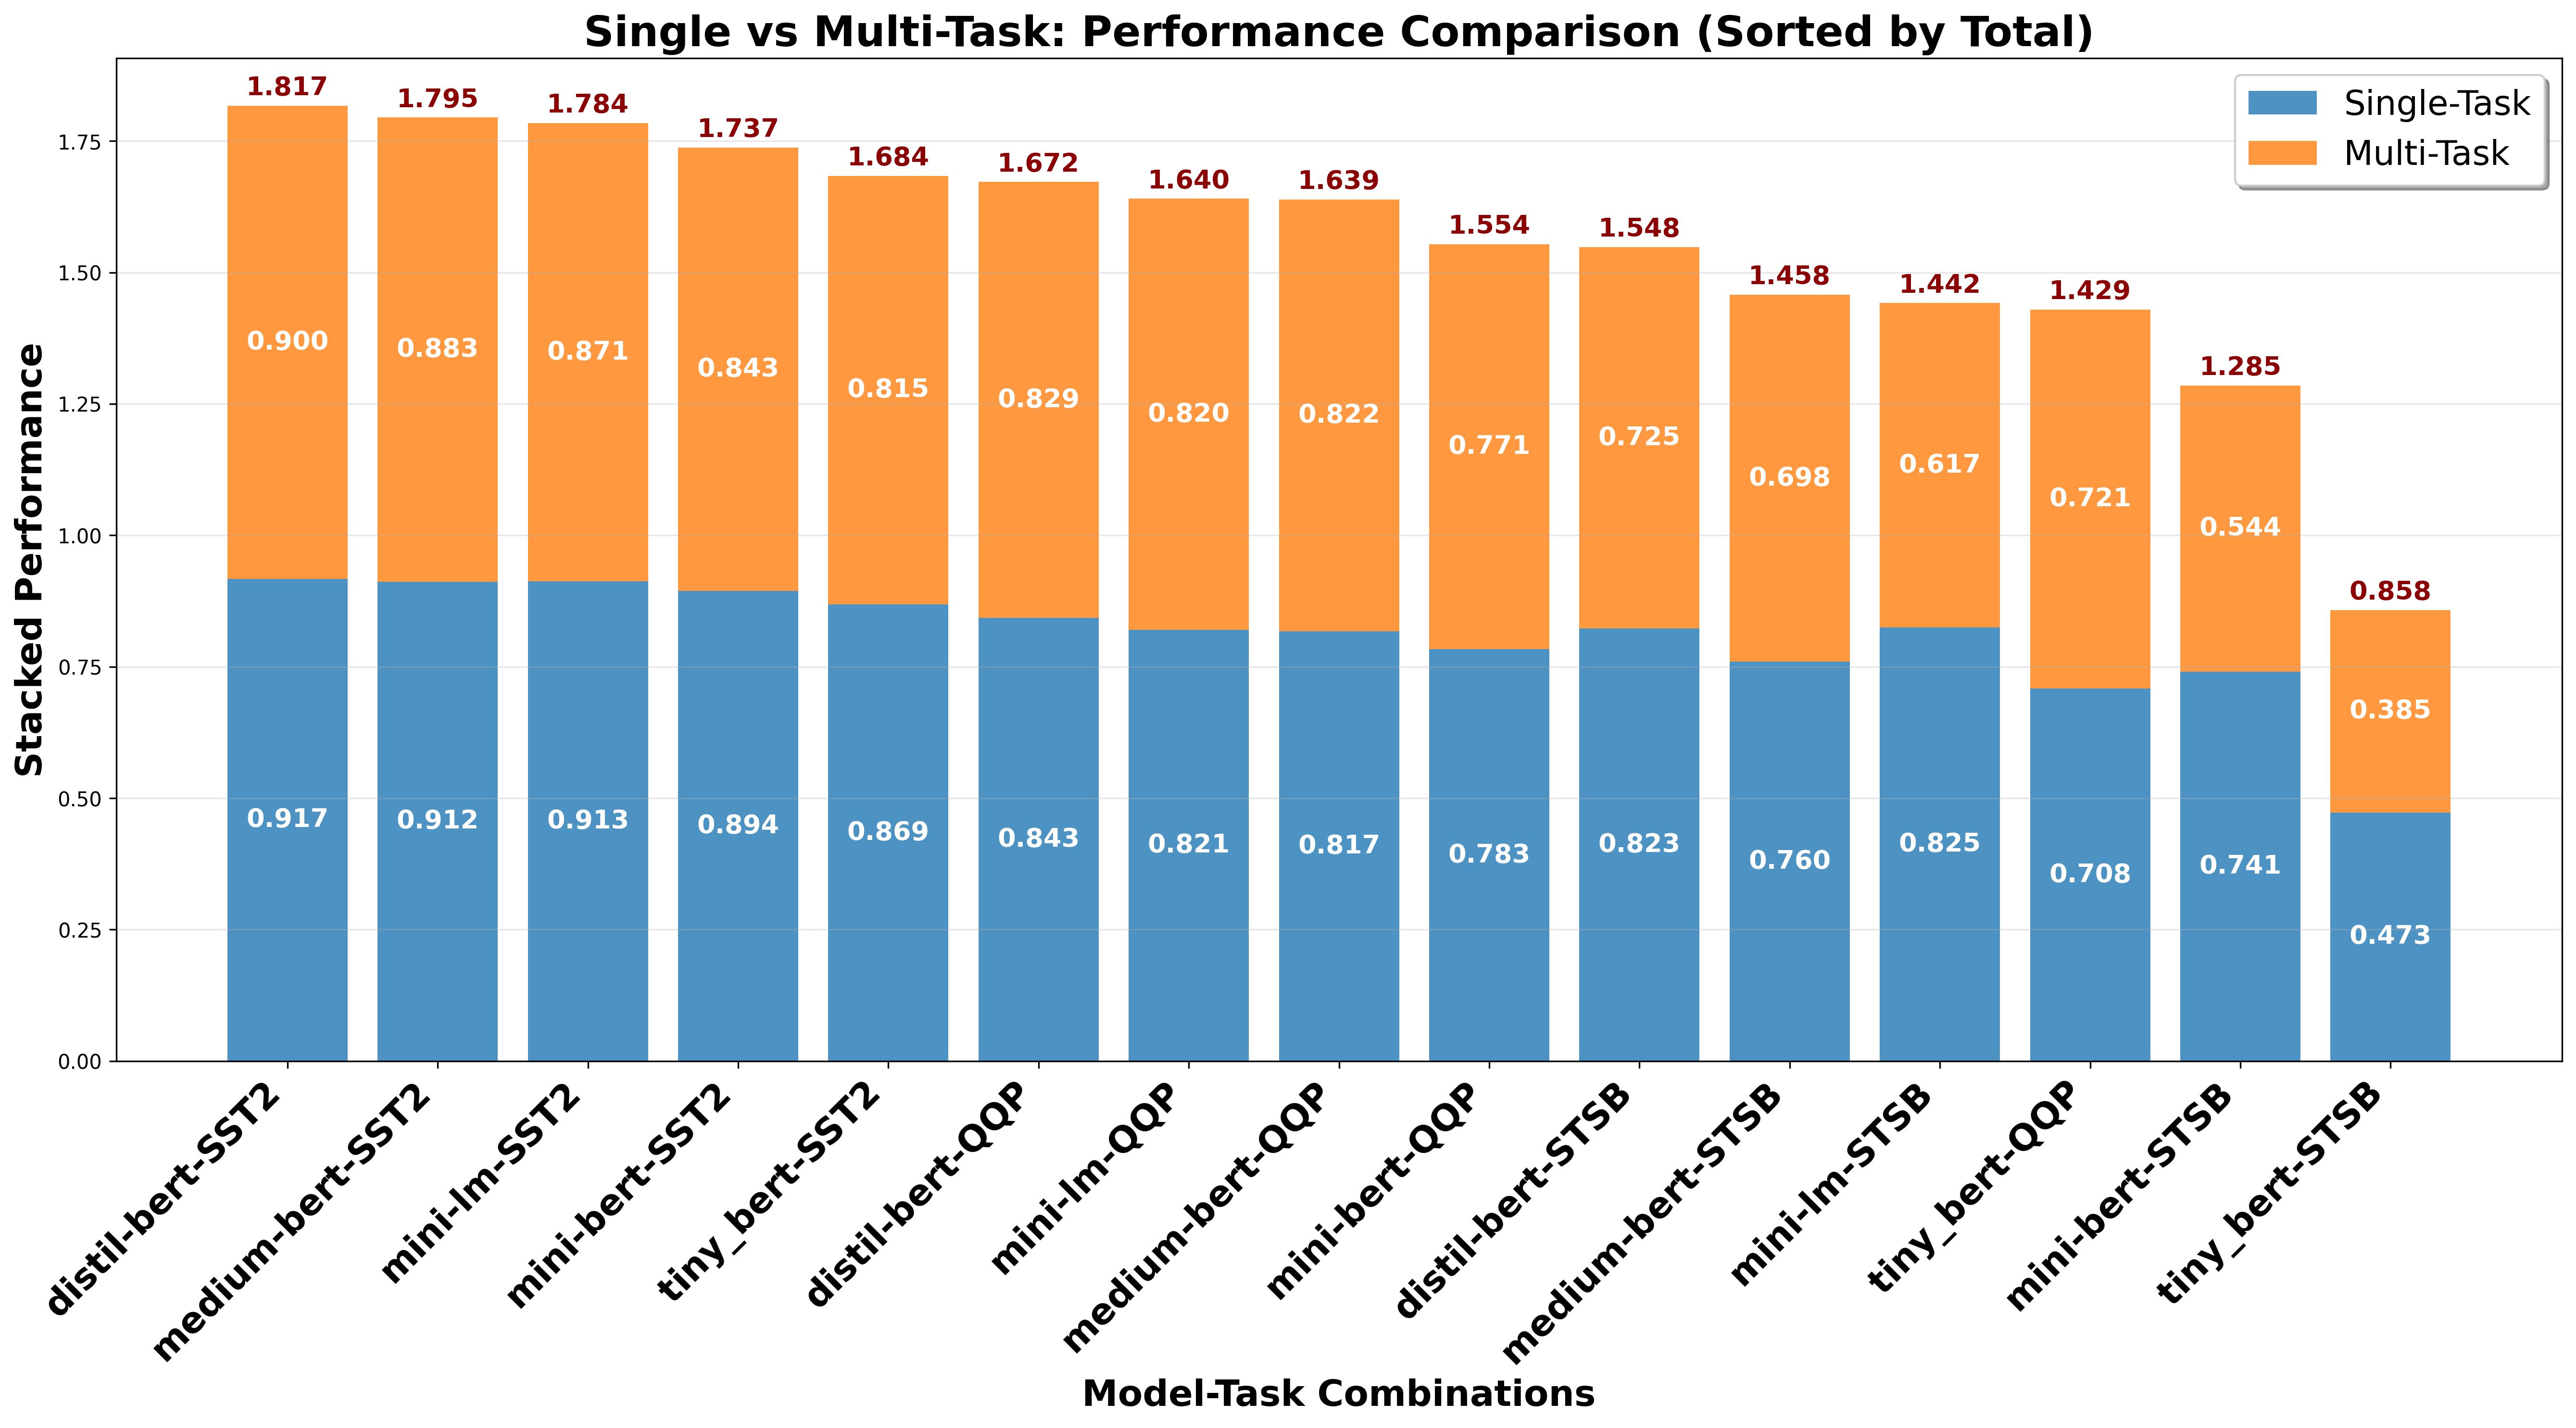
\includegraphics[width=\textwidth]{../plots/single_vs_multitask_stacked_performance_balanced.png}
        \caption{Single vs Multi-Task Performance across 5 model architectures}
    \end{minipage}
    \hfill
    \begin{minipage}{0.45\textwidth}
        \centering
        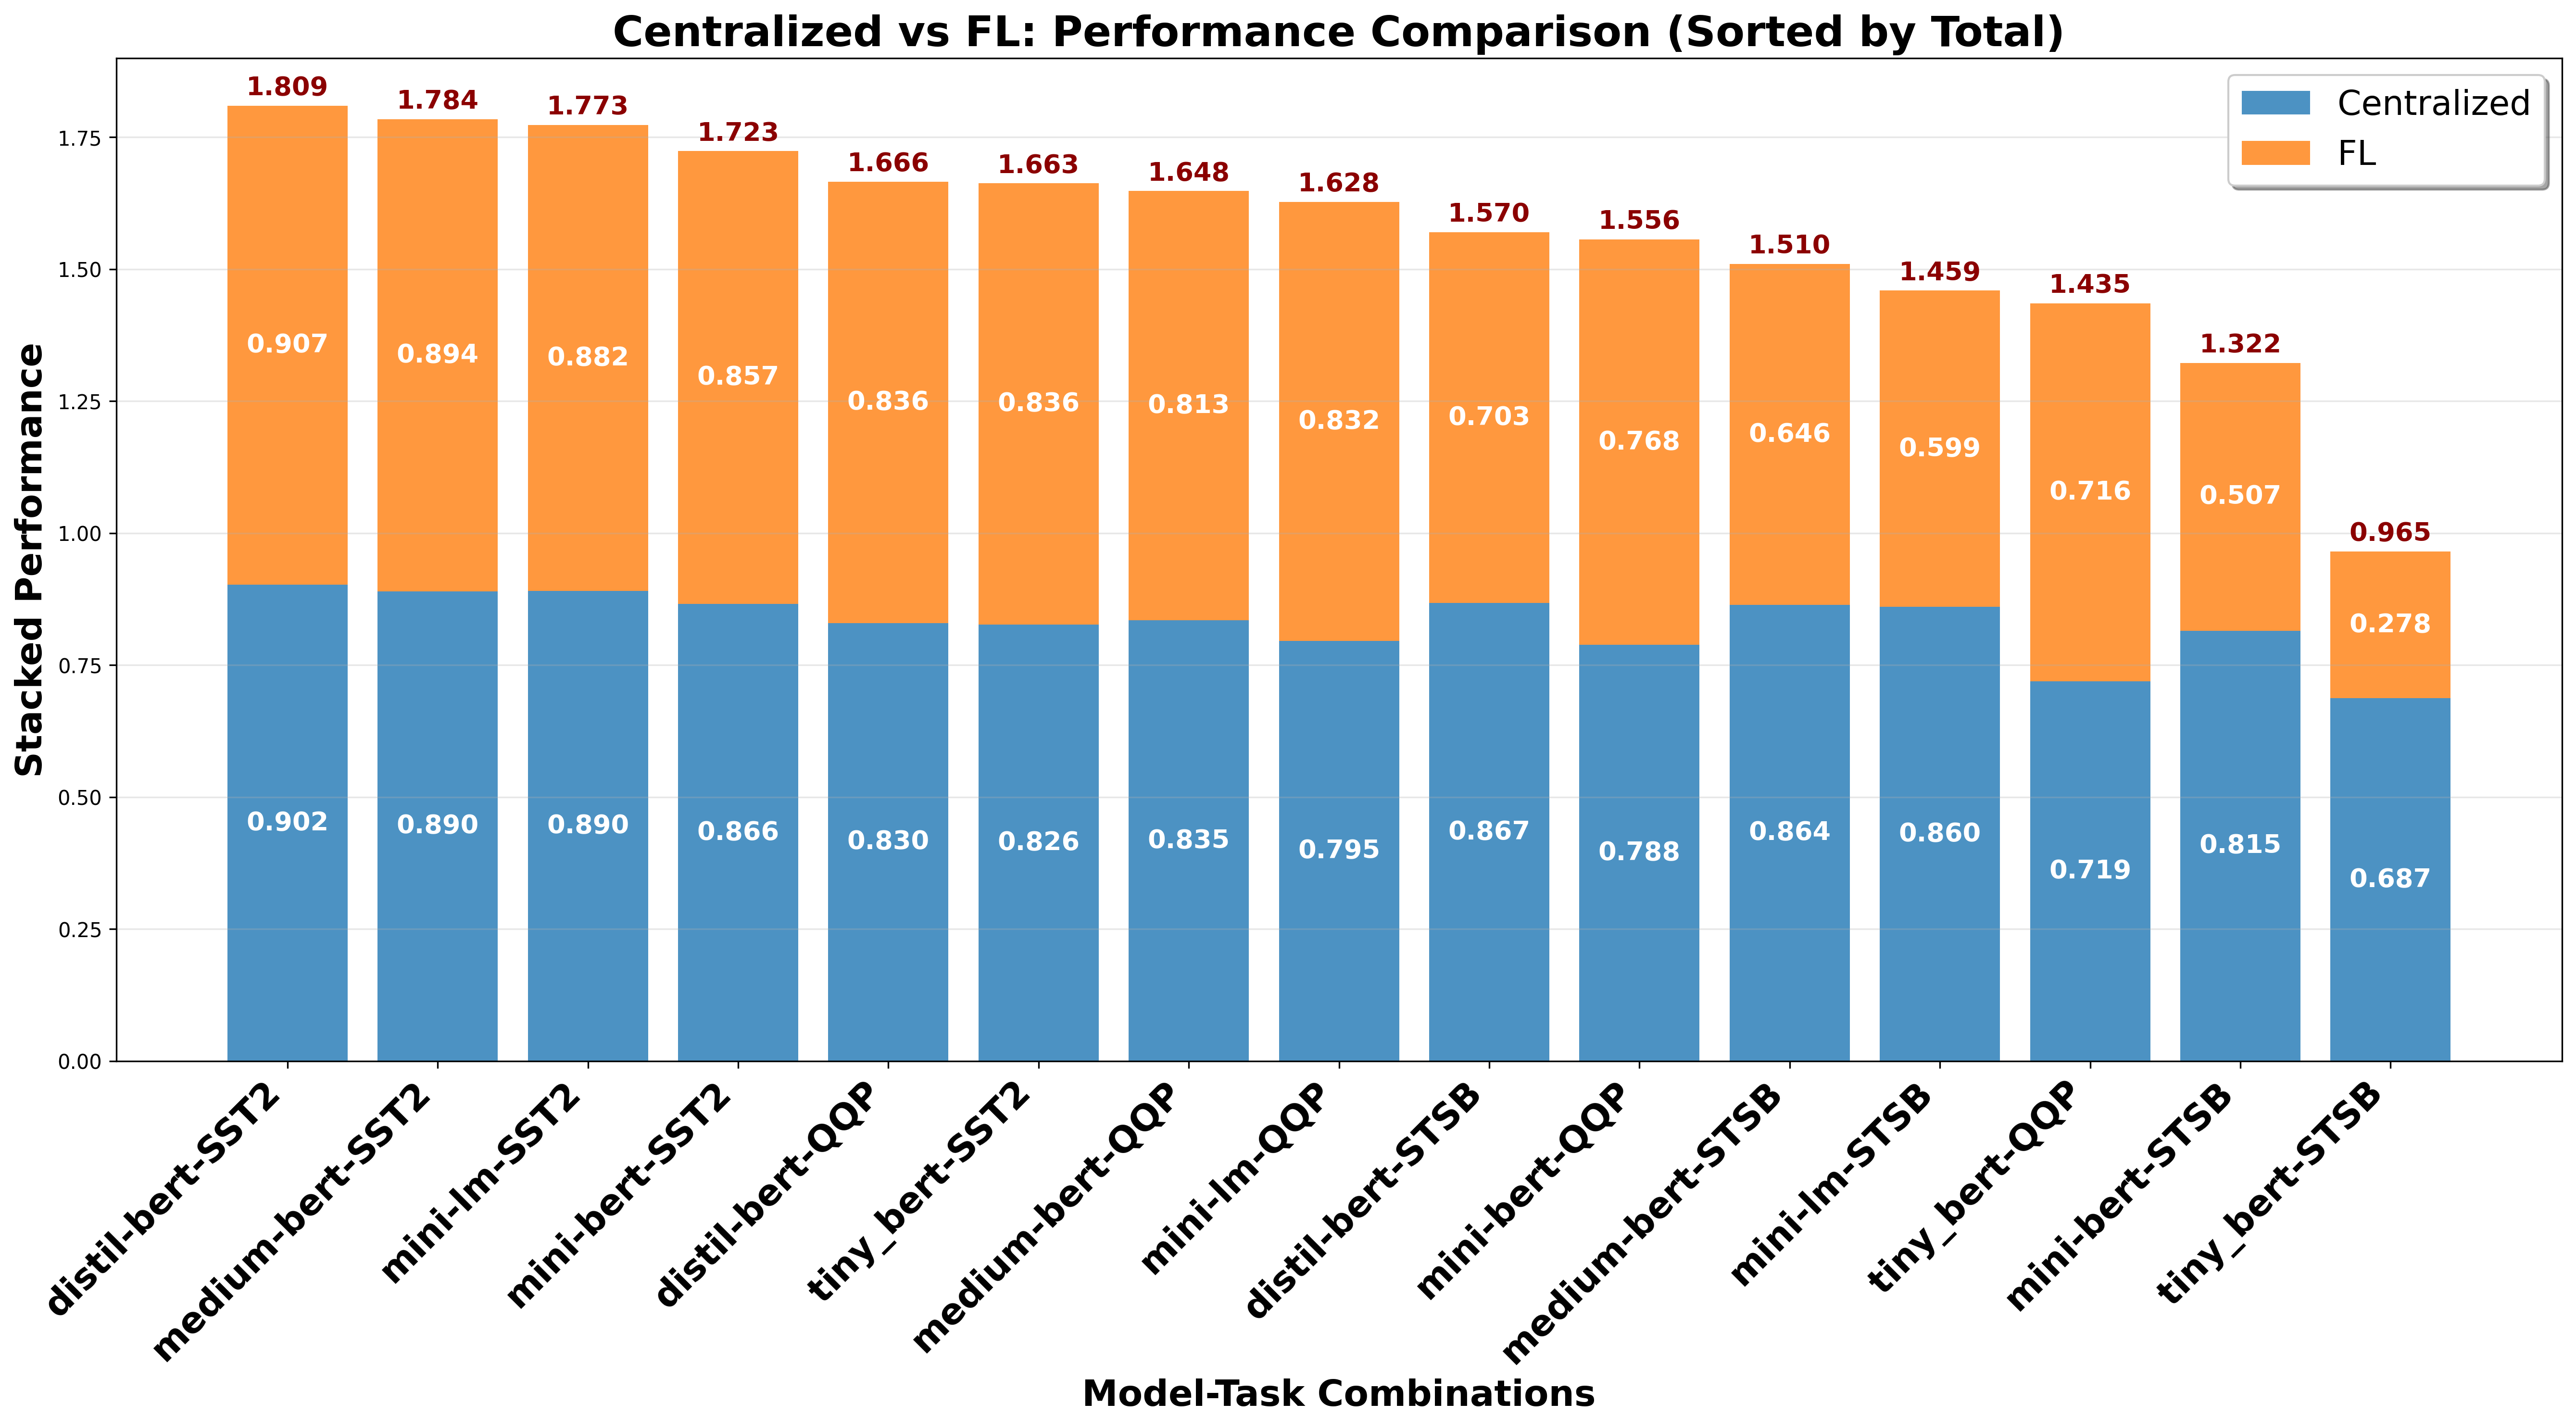
\includegraphics[width=\textwidth]{../plots/centralized_vs_fl_stacked_performance_balanced.png}
        \caption{Centralized vs FL Performance comparison}
    \end{minipage}
    \label{fig:performance_comparison}
\end{figure}

\begin{table}[h]
    \centering
    \caption{Single vs Multi-Task Performance Metrics}
    \begin{tabular}{|l|c|c|c|c|c|c|}
        \hline
        \textbf{Model} & \textbf{Task} & \textbf{Single} & \textbf{Multi} & \textbf{Total} & \textbf{Diff} & \textbf{\% Diff} \\
        \hline
        distil-bert & SST2 & 0.9174 & 0.8997 & 1.8171 & -0.0177 & -1.93\% \\
        medium-bert & SST2 & 0.9117 & 0.8830 & 1.7947 & -0.0287 & -3.14\% \\
        mini-lm & SST2 & 0.9128 & 0.8710 & 1.7838 & -0.0418 & -4.58\% \\
        mini-bert & SST2 & 0.8939 & 0.8435 & 1.7374 & -0.0504 & -5.64\% \\
        tiny\_bert & SST2 & 0.8687 & 0.8151 & 1.6838 & -0.0536 & -6.17\% \\
        \hline
    \end{tabular}
    \label{tab:multitask_metrics}
\end{table}

As shown in Figure~\ref{fig:performance_comparison}, our comprehensive evaluation reveals significant insights into multi-task learning dynamics. The Single vs Multi-Task Performance comparison demonstrates that single-task learning consistently outperforms multi-task learning across most model-task combinations. Table~\ref{tab:multitask_metrics} quantifies this performance degradation, which ranges from -1.93\% for distil-bert to -6.17\% for tiny\_bert on the SST2 task. This indicates prevalent negative transfer effects in multi-task scenarios.

The Centralized vs FL Performance comparison (Figure~\ref{fig:performance_comparison}) reveals that federated learning maintains competitive performance with centralized training for classification tasks. Table~\ref{tab:fl_metrics} shows minimal performance differences, with FL achieving slight improvements for some models (tiny\_bert: +1.22\%) and minor degradation for others (mini-bert: -0.96\%). However, the most significant finding is the substantial performance drop for semantic similarity tasks under FL, particularly evident in the STSB task where performance degradation can exceed 25\% for larger models.

Key findings from our analysis indicate that larger models (distil-bert, medium-bert) demonstrate better multi-task adaptation capabilities, while the STSB task consistently shows the highest sensitivity to multi-task interference. This suggests that task complexity and semantic requirements significantly impact the effectiveness of multi-task learning approaches.

\subsubsection{Impact of Federated Learning}

\begin{figure}[h]
    \centering
    \begin{minipage}{0.45\textwidth}
        \centering
        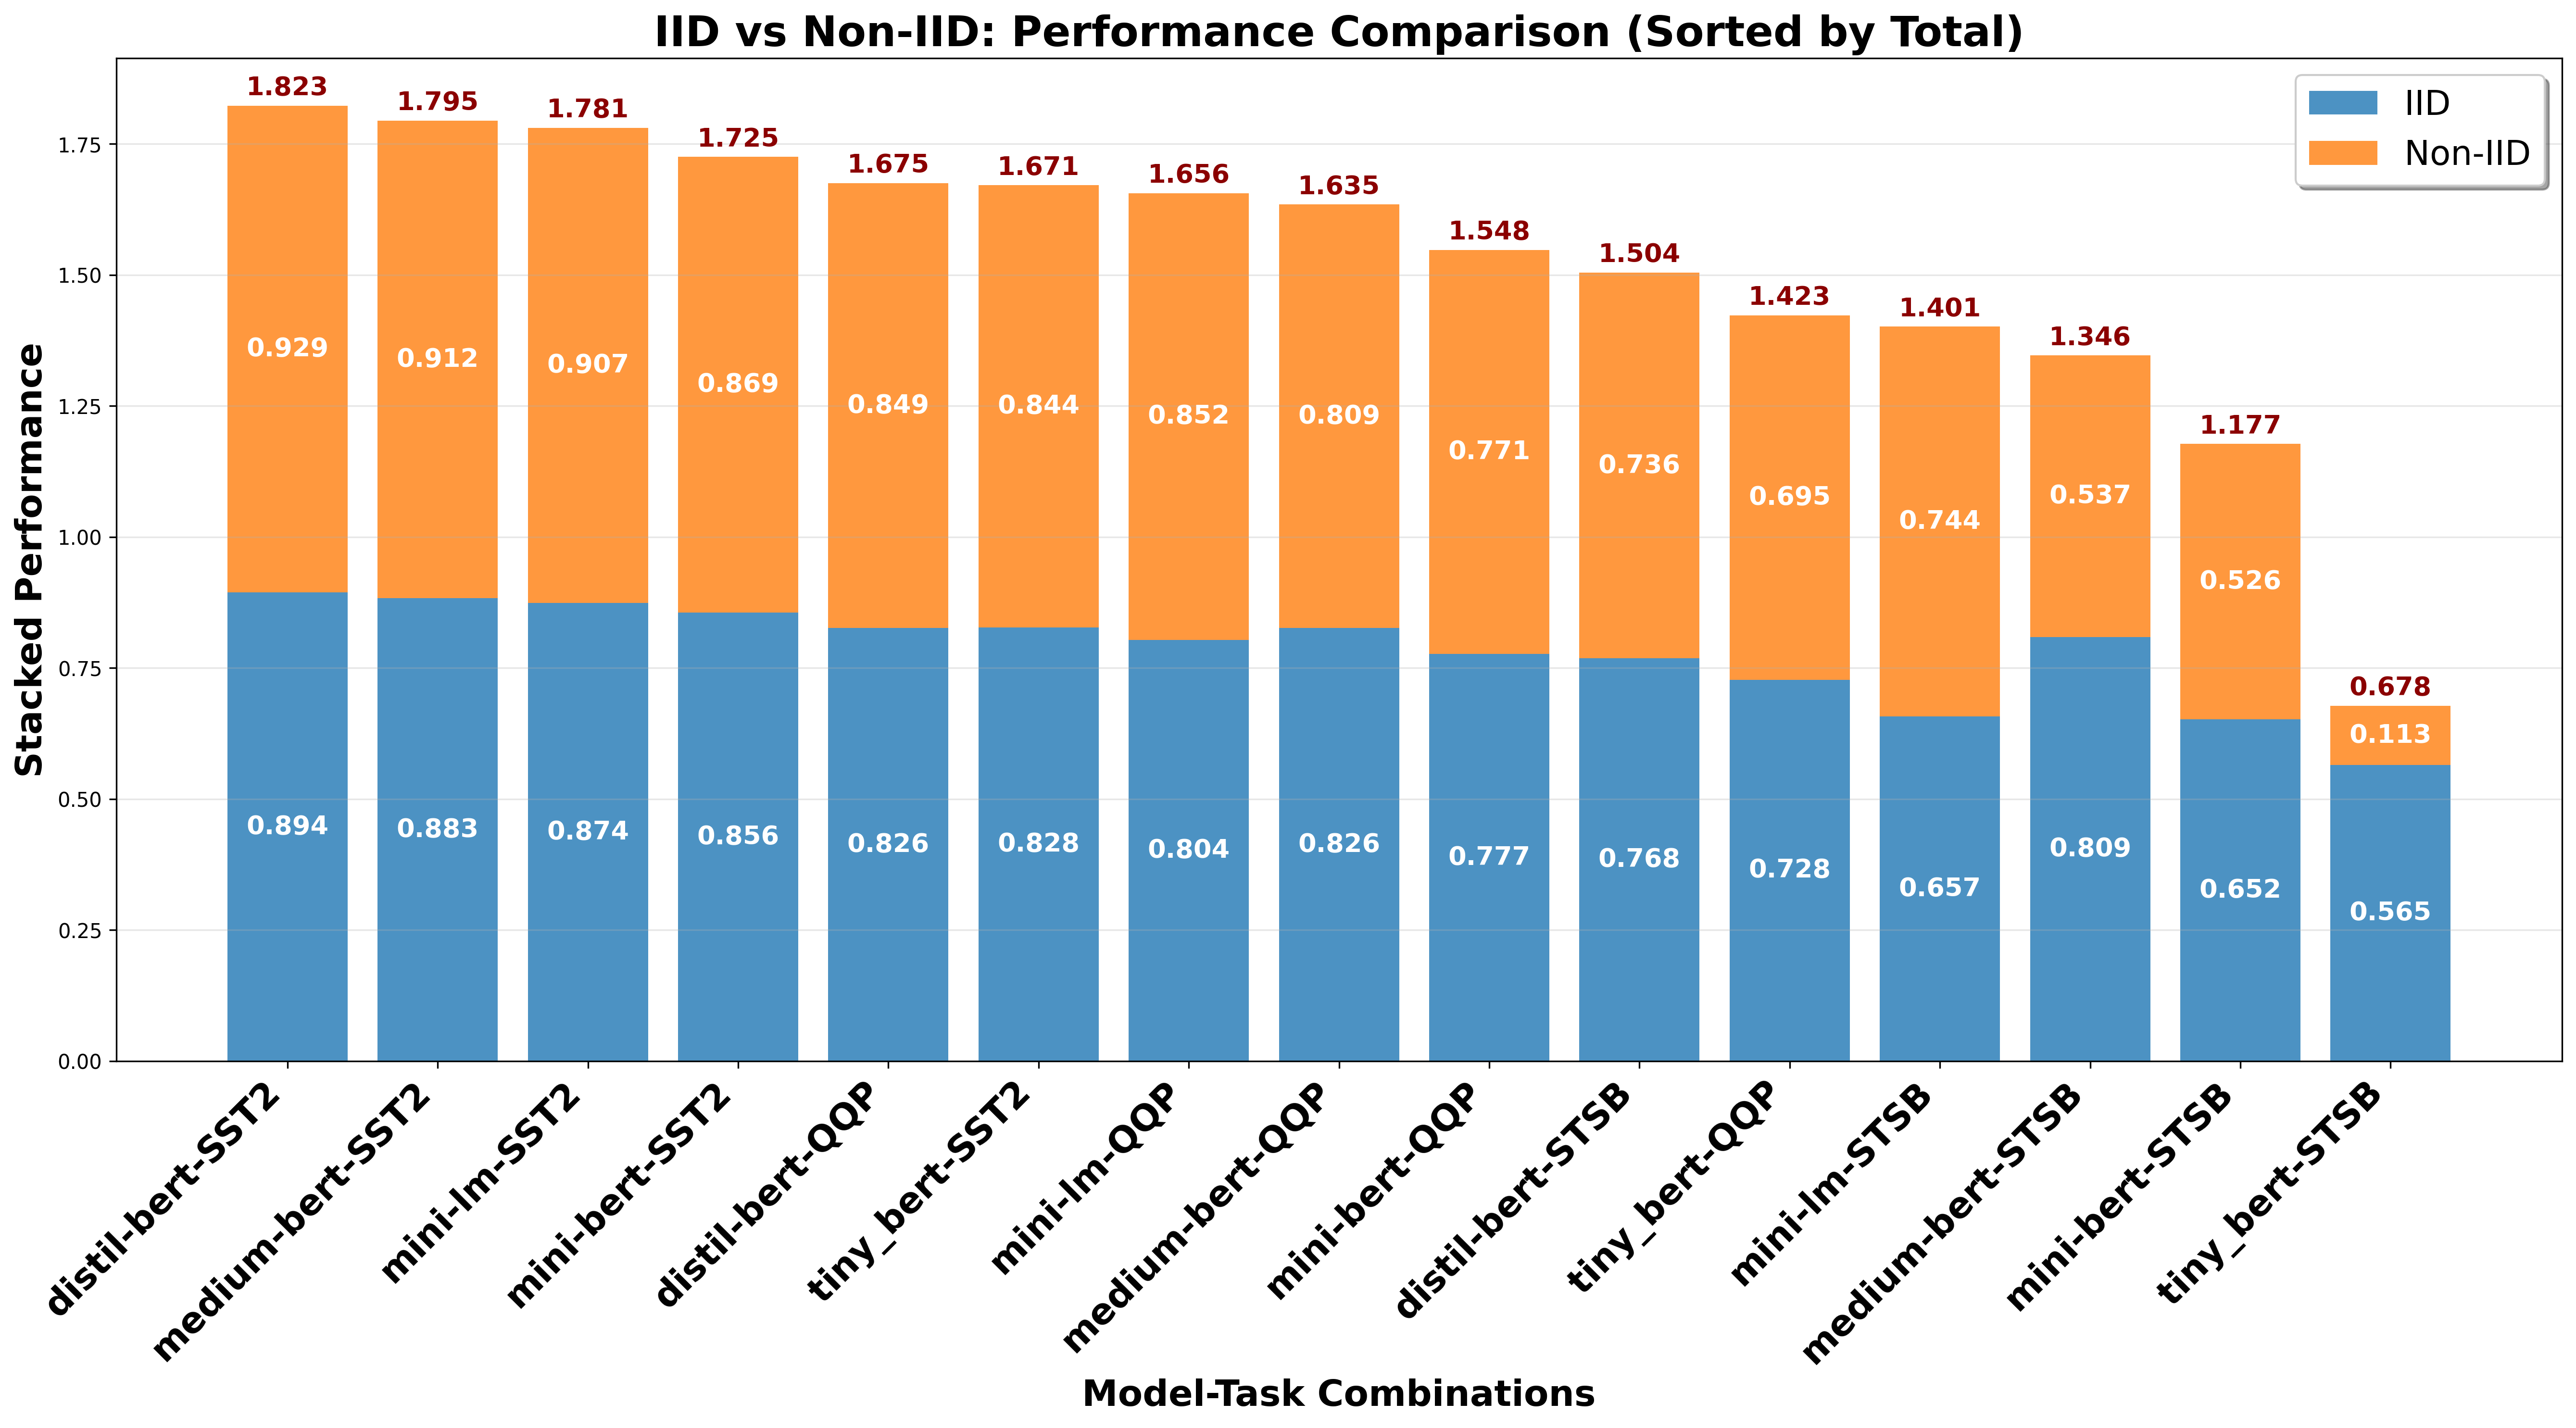
\includegraphics[width=\textwidth]{../plots/iid_vs_noniid_stacked_performance_balanced.png}
        \caption{IID vs Non-IID Performance across 5 models}
    \end{minipage}
    \hfill
    \begin{minipage}{0.45\textwidth}
        \centering
        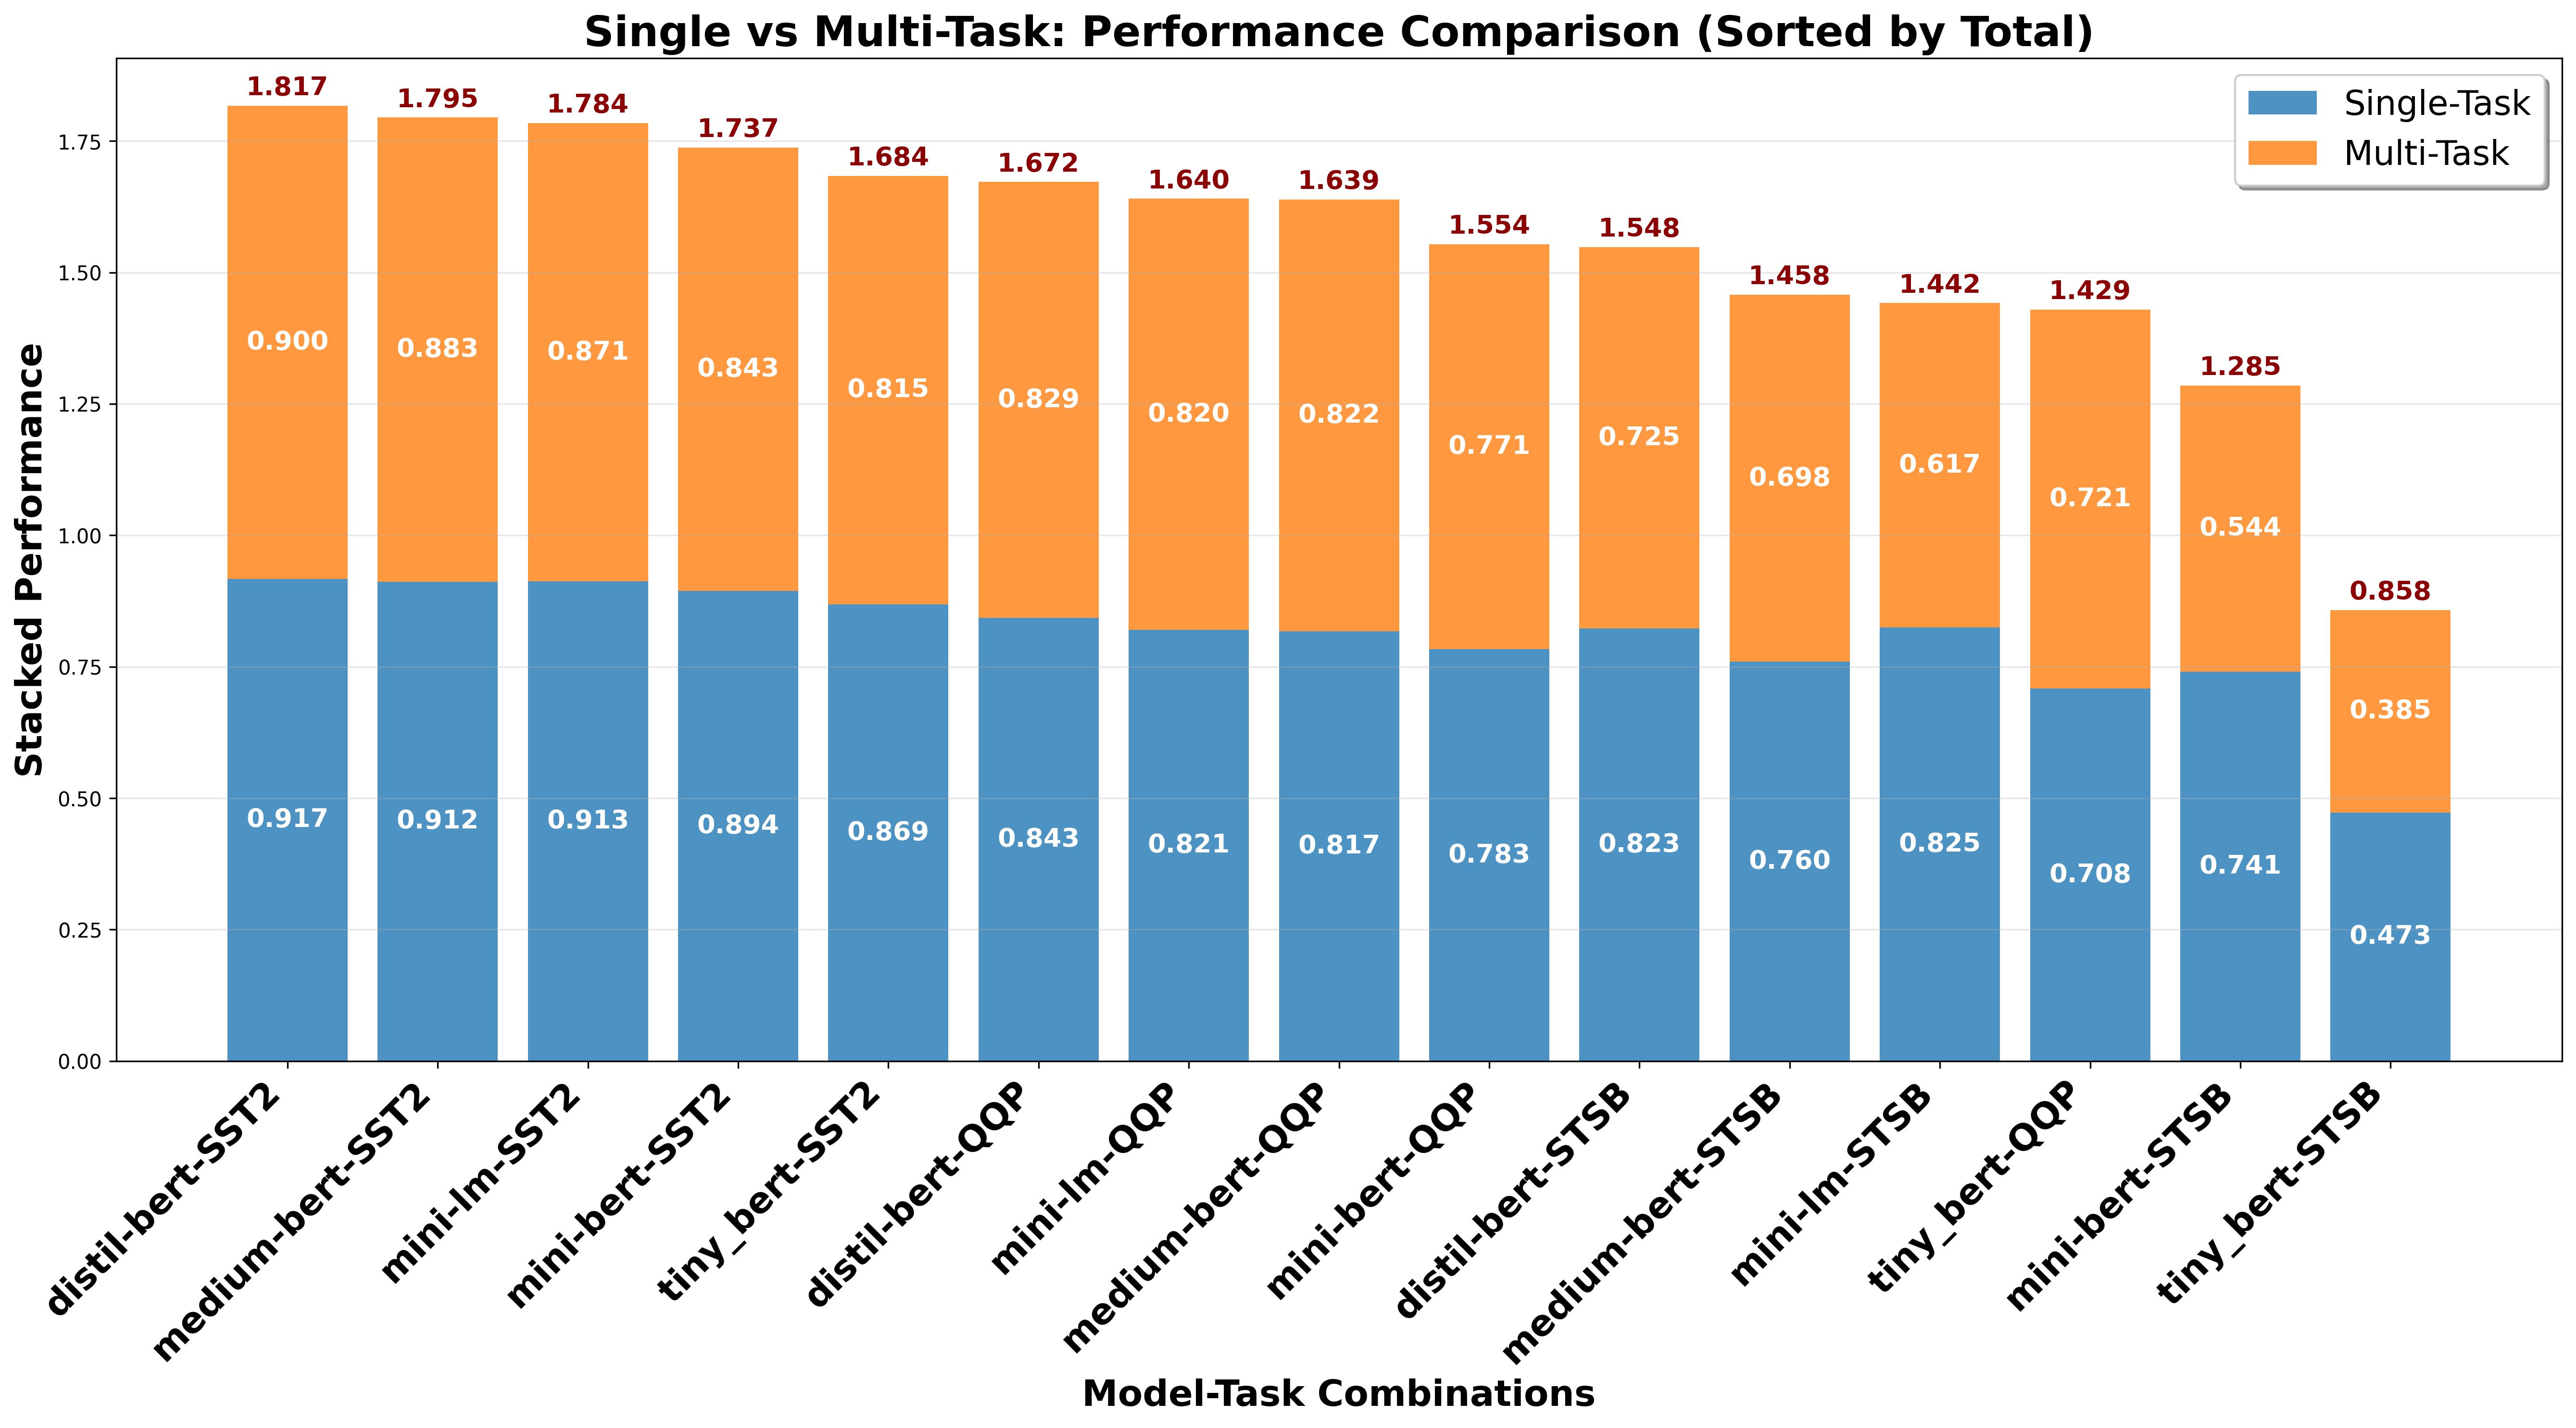
\includegraphics[width=\textwidth]{../plots/single_vs_multitask_stacked_performance_balanced.png}
        \caption{Task Transfer Effects: Single vs Multi-Task}
    \end{minipage}
    \label{fig:fl_impact}
\end{figure}

\begin{table}[h]
    \centering
    \caption{Centralized vs Federated Learning Performance Metrics}
    \begin{tabular}{|l|c|c|c|c|c|c|}
        \hline
        \textbf{Model} & \textbf{Task} & \textbf{Centralized} & \textbf{FL} & \textbf{Total} & \textbf{Diff} & \textbf{\% Diff} \\
        \hline
        distil-bert & SST2 & 0.9019 & 0.9074 & 1.8093 & 0.0055 & 0.60\% \\
        medium-bert & SST2 & 0.8899 & 0.8939 & 1.7838 & 0.0040 & 0.45\% \\
        mini-lm & SST2 & 0.8905 & 0.8822 & 1.7727 & -0.0083 & -0.93\% \\
        mini-bert & SST2 & 0.8658 & 0.8575 & 1.7233 & -0.0083 & -0.96\% \\
        tiny\_bert & SST2 & 0.8263 & 0.8363 & 1.6626 & 0.0101 & 1.22\% \\
        \hline
    \end{tabular}
    \label{tab:fl_metrics}
\end{table}

The impact of federated learning on model performance is multifaceted, as illustrated in Figure~\ref{fig:fl_impact}. Our analysis of data heterogeneity and client variability reveals several critical patterns. First, FL demonstrates competitive performance with centralized training for classification tasks (SST2, QQP), as evidenced by the minimal performance differences shown in Table~\ref{tab:fl_metrics}. However, the IID vs Non-IID Performance comparison (Figure~\ref{fig:fl_impact}) highlights significant robustness challenges across different model architectures.

Figure~\ref{fig:iid_performance} provides detailed insights into model robustness to distribution shifts. The stacked visualization reveals that different tasks exhibit varying sensitivity to non-IID data distributions, with semantic similarity tasks showing the highest vulnerability. This finding is consistent across all five model architectures, suggesting inherent challenges in federated learning for complex semantic understanding tasks.

The Task Transfer Effects visualization (Figure~\ref{fig:fl_impact}) further demonstrates that data heterogeneity impacts vary significantly by task complexity and model architecture. Our observations indicate that client variability effects are more pronounced in smaller models (mini-bert, tiny\_bert), which struggle to maintain performance consistency across diverse data distributions. This suggests that model capacity plays a crucial role in federated learning robustness.

\begin{figure}[h]
    \centering
    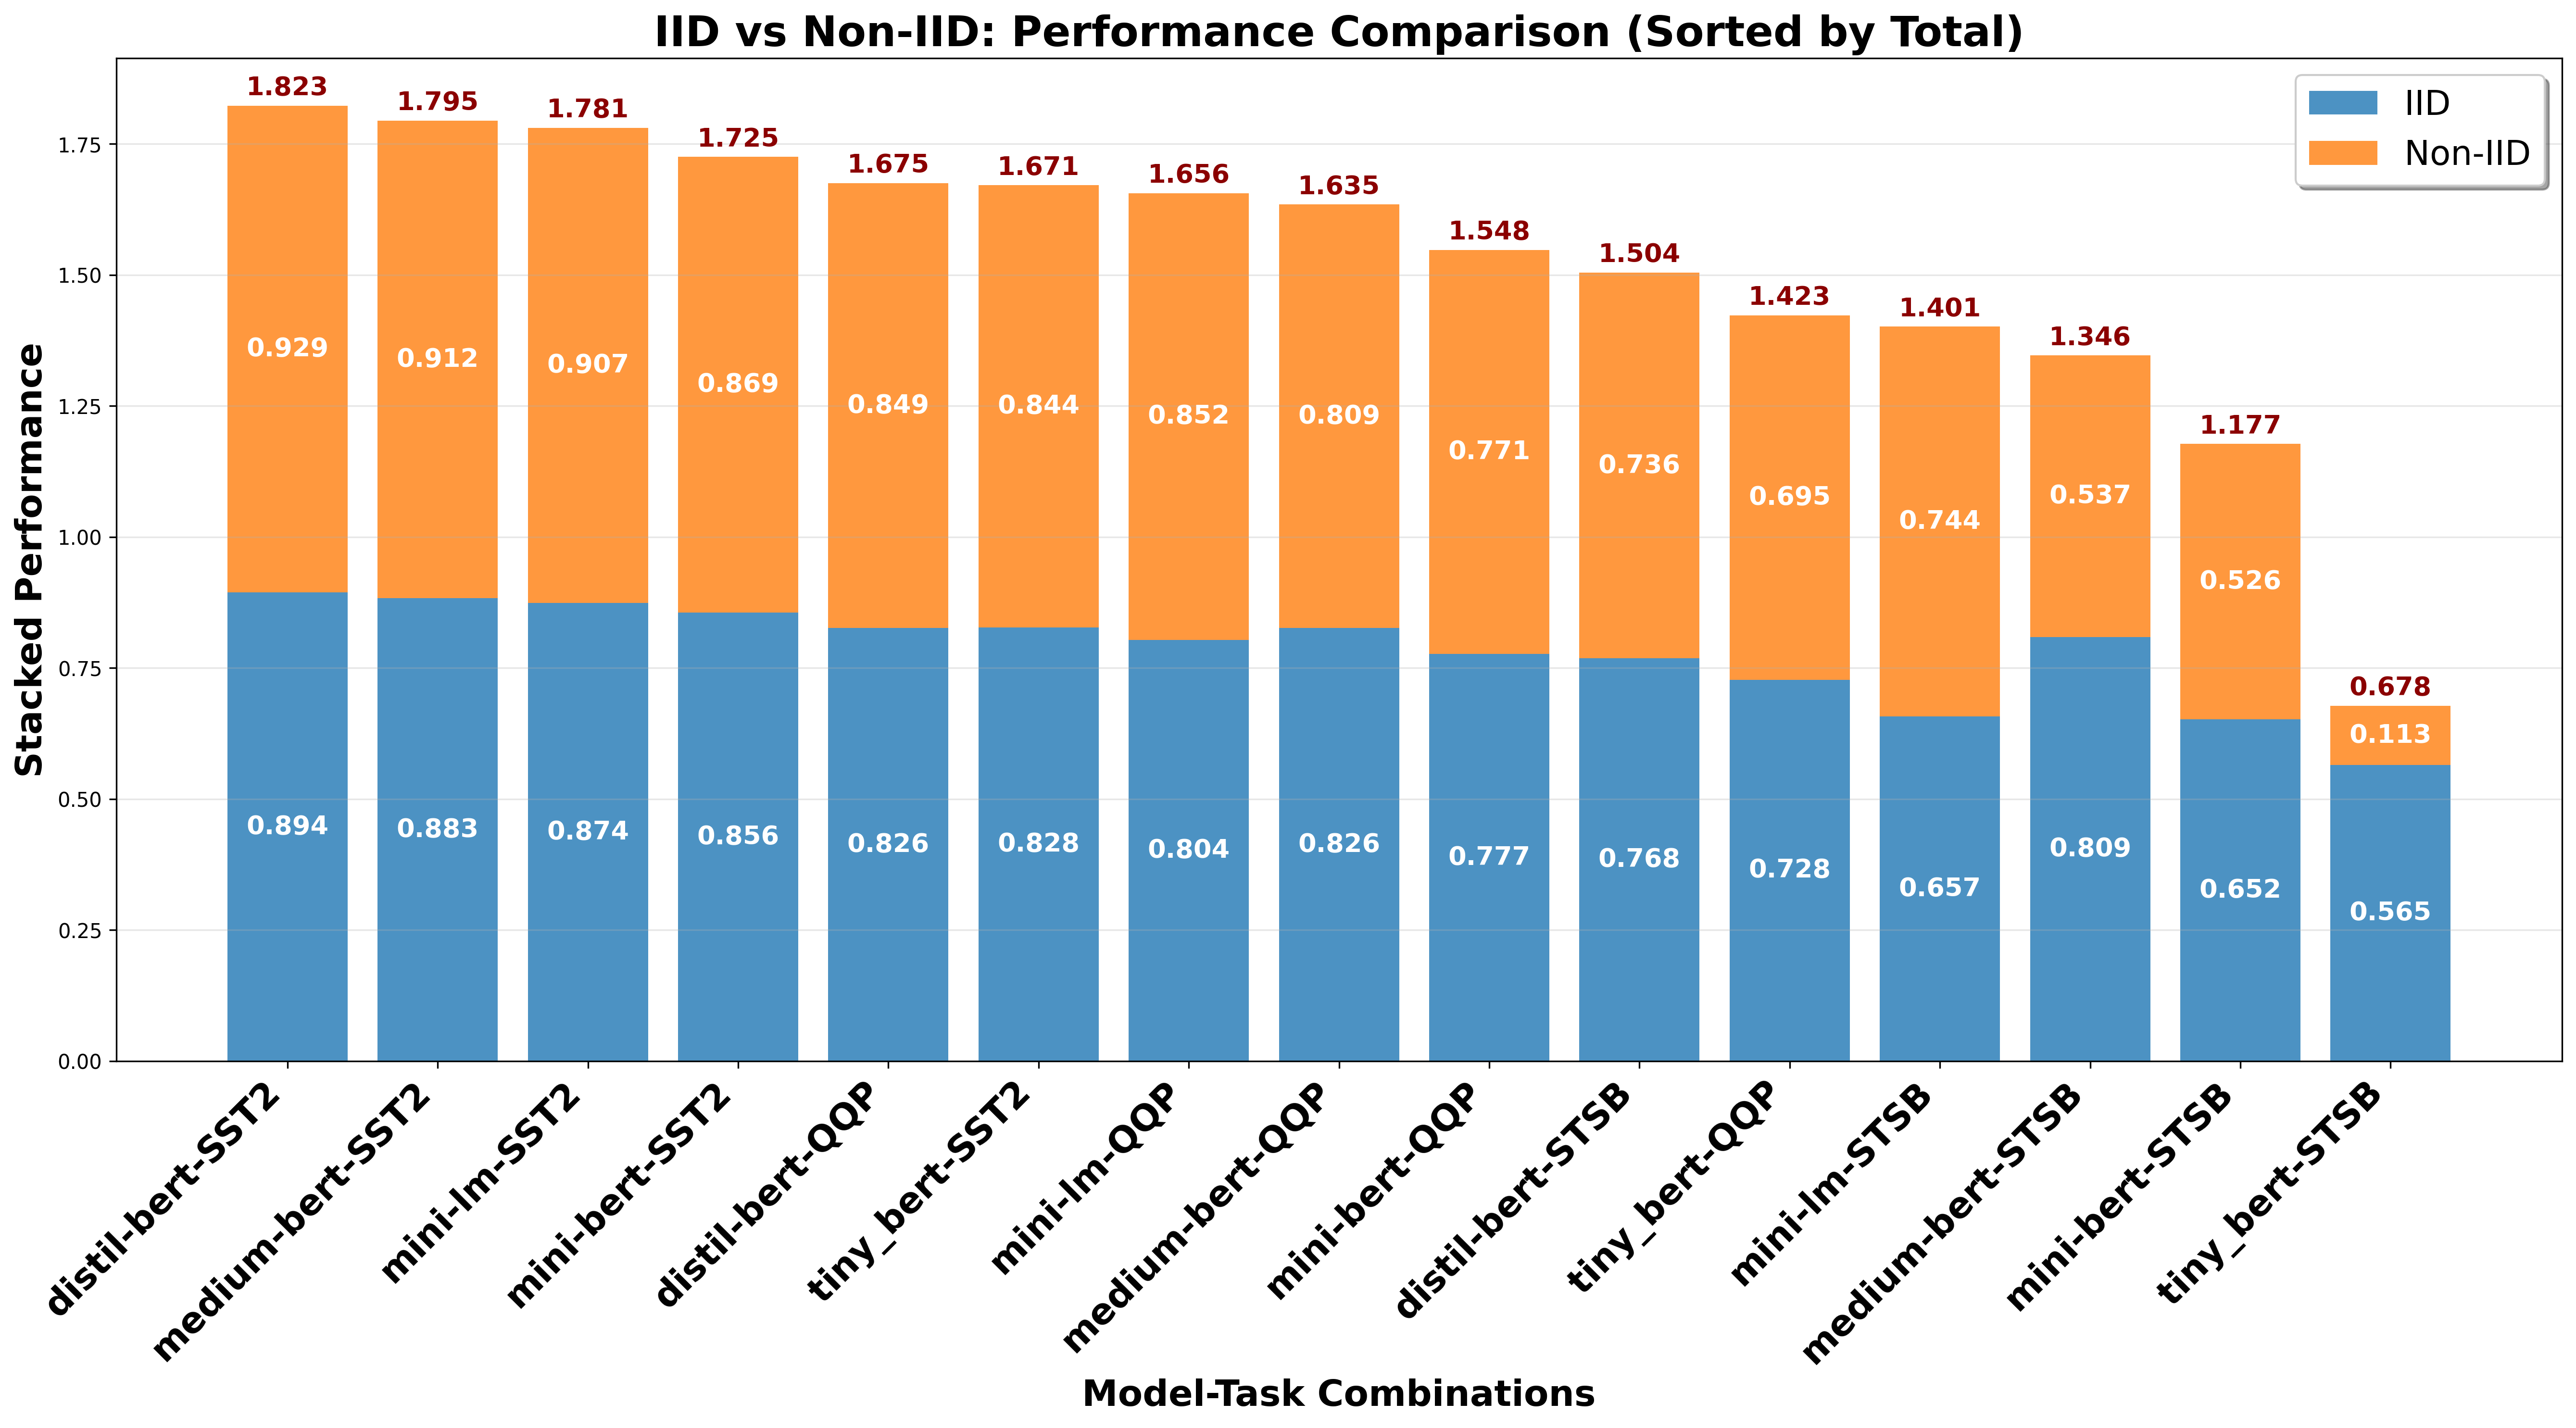
\includegraphics[width=0.5\textwidth]{../plots/iid_vs_noniid_stacked_performance_balanced.png}
    \caption{IID vs Non-IID: Stacked Performance Comparison revealing model robustness to distribution shifts. Height ratios indicate different sensitivity patterns across tasks and model architectures.}
    \label{fig:iid_performance}
\end{figure}

\subsubsection{Efficiency Analysis}

Our efficiency analysis reveals significant trade-offs between communication cost, training time, and model performance. As depicted in Figure~\ref{fig:training_time}, the line plot visualization clearly shows training time patterns across all experimental dimensions. The comprehensive line plot reveals FL's communication overhead with distinct gaps between Centralized and FL lines, while also showing how IID vs Non-IID and Single vs Multi-task comparisons affect training efficiency. Table~\ref{tab:training_efficiency} quantifies the training overhead, with FL requiring 2.39-3.85x more time than centralized training for most models. Notably, distil-bert exhibits the highest overhead (21,137 seconds additional), while tiny\_bert is the only model where FL training is actually faster (0.97x ratio).

The resource usage analysis, illustrated in Figure~\ref{fig:resource_usage}, demonstrates FL's distributed resource efficiency advantages using line plots that clearly reveal trends across all experimental dimensions. The line plot visualization shows all six categories (Centralized, FL, IID, Non-IID, Single, Multi) with different line styles and markers, making patterns and trends more visible than bar charts. Table~\ref{tab:resource_efficiency} quantifies the centralized vs FL relationship, showing that FL reduces individual client resource usage by 77-93\% compared to centralized approaches, with mini-bert achieving the highest efficiency (0.07x ratio). This dramatic reduction in per-client resource requirements makes FL particularly attractive for deployment on resource-constrained devices.

These efficiency metrics reveal important insights for practical deployment. While FL introduces significant communication overhead and longer training times, the distributed resource efficiency gains offset these costs in many scenarios. The model-specific variations suggest that optimal deployment strategies should consider both performance requirements and resource constraints when choosing between centralized and federated approaches.

\begin{figure}[h]
    \centering
    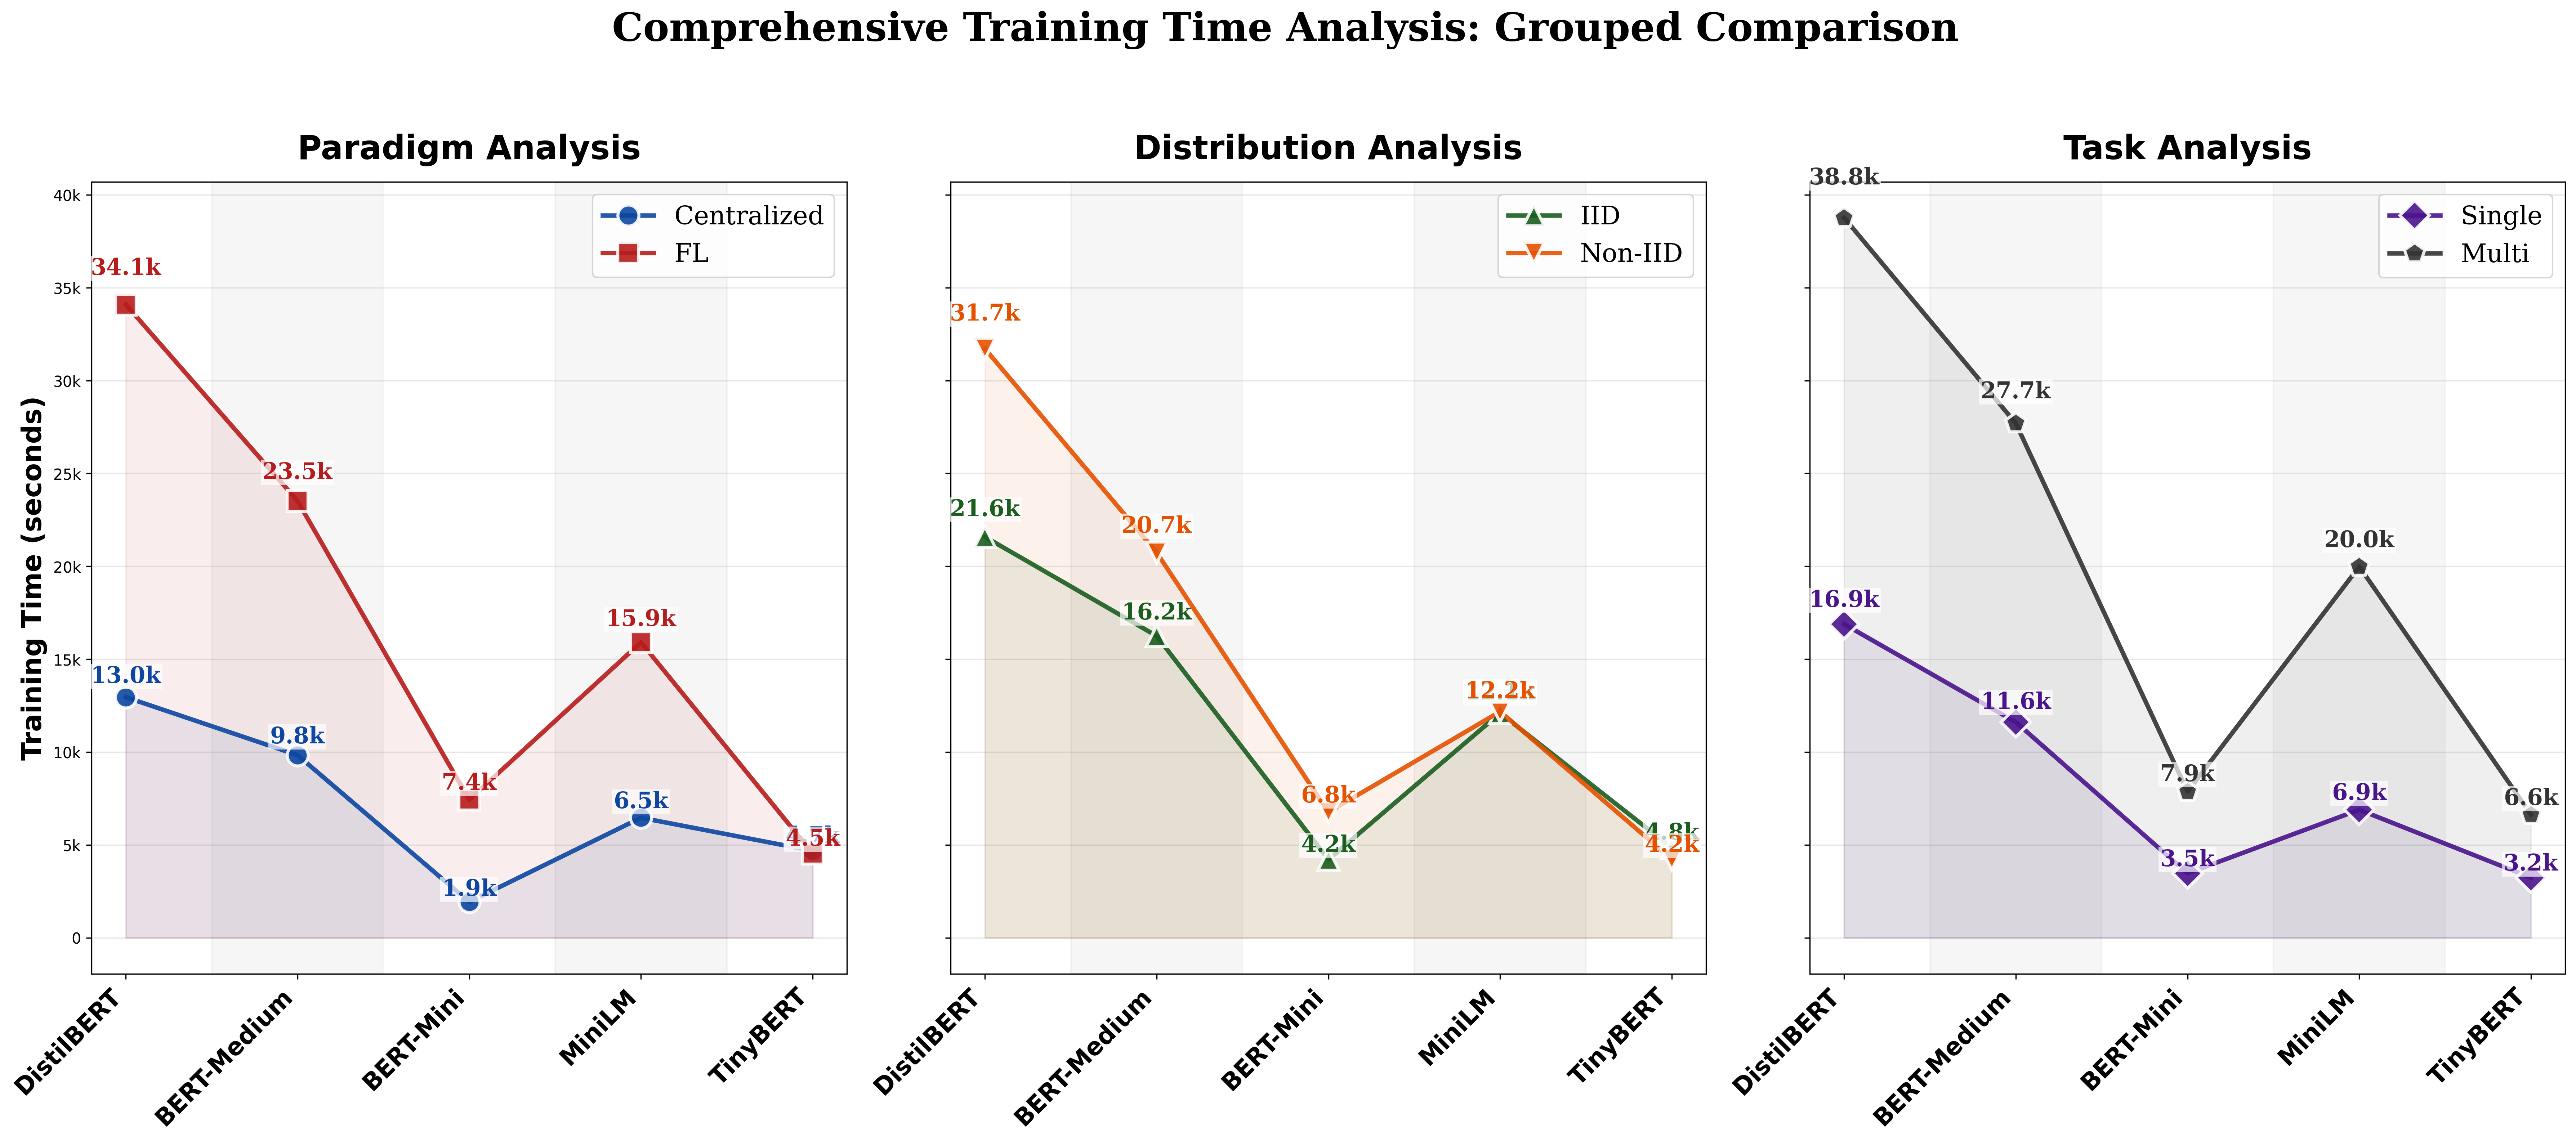
\includegraphics[width=0.9\textwidth]{../plots/line_training_time_balanced.png}
    \caption{Comprehensive Training Time Analysis using line plots to show trends across all six categories (Centralized, FL, IID, Non-IID, Single, Multi) for clear pattern visualization}
    \label{fig:training_time}
\end{figure}

\begin{table}[h]
    \centering
    \caption{Training Time Efficiency Analysis}
    \begin{tabular}{|l|c|c|c|c|c|}
        \hline
        \textbf{Model} & \textbf{Centralized (s)} & \textbf{FL (s)} & \textbf{Ratio} & \textbf{Overhead (s)} \\
        \hline
        distil-bert & 12,954 & 34,091 & 2.63 & 21,137 \\
        medium-bert & 9,834 & 23,517 & 2.39 & 13,682 \\
        mini-lm & 6,464 & 15,909 & 2.46 & 9,445 \\
        mini-bert & 1,933 & 7,432 & 3.85 & 5,499 \\
        tiny\_bert & 4,684 & 4,539 & 0.97 & -145 \\
        \hline
    \end{tabular}
    \label{tab:training_efficiency}
\end{table}

\textbf{Model Size and Resource Usage:}

\begin{figure}[h]
    \centering
    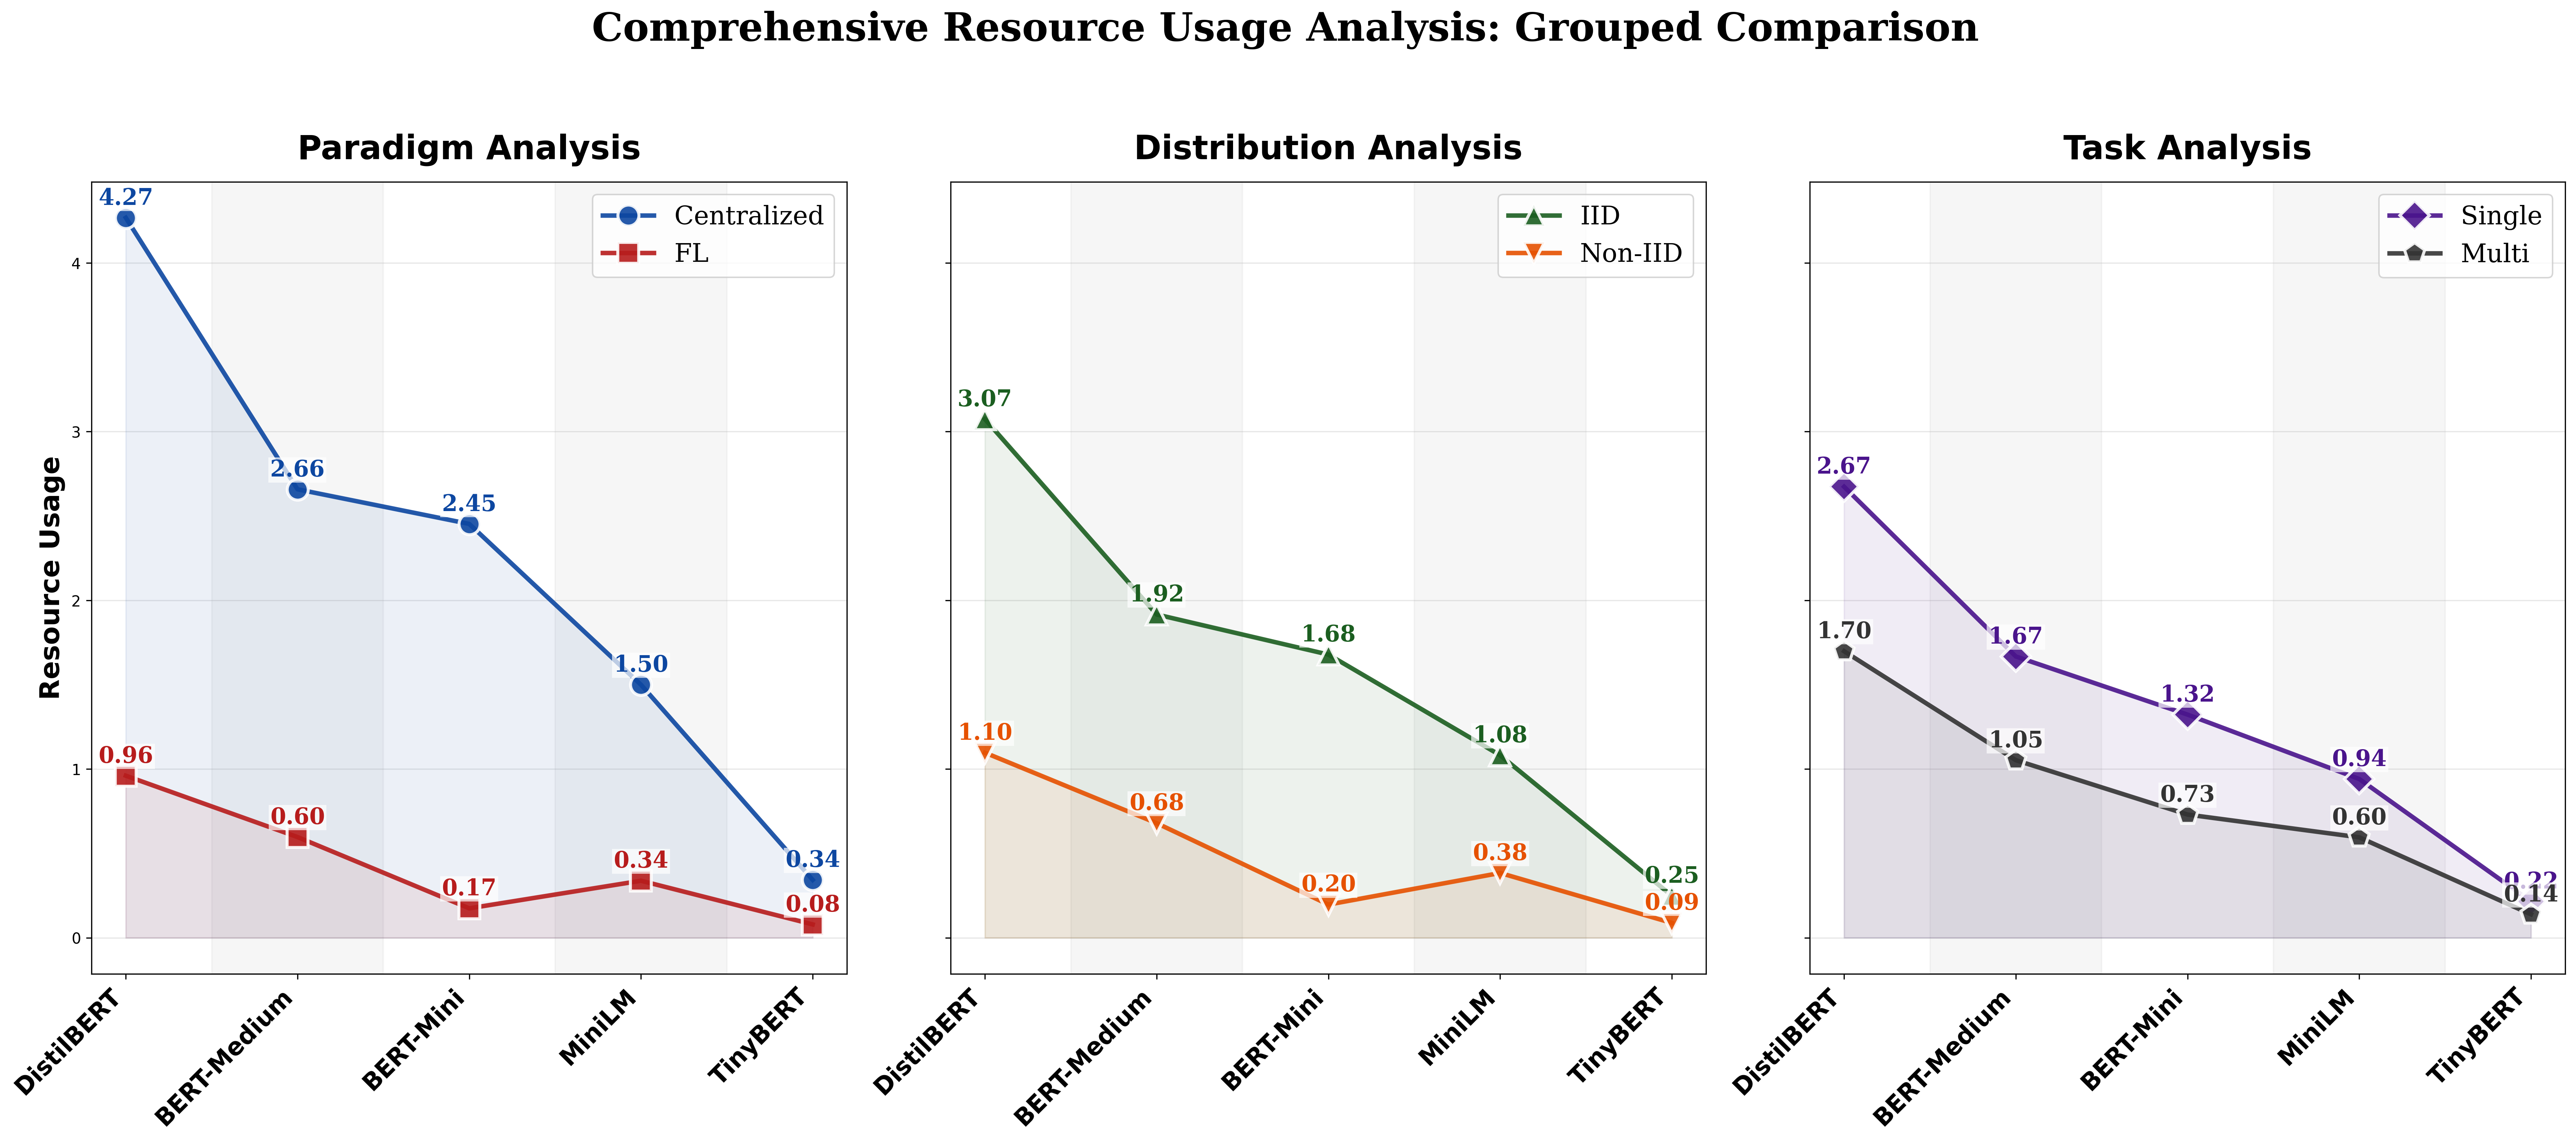
\includegraphics[width=0.9\textwidth]{../plots/line_resource_usage_balanced.png}
    \caption{Comprehensive Resource Usage Analysis using line plots to show trends across all six categories (Centralized, FL, IID, Non-IID, Single, Multi) for clear pattern visualization}
    \label{fig:resource_usage}
\end{figure}

\begin{table}[h]
    \centering
    \caption{Resource Usage Analysis}
    \begin{tabular}{|l|c|c|c|c|c|}
        \hline
        \textbf{Model} & \textbf{Centralized} & \textbf{FL} & \textbf{Total} & \textbf{Ratio} & \textbf{Savings} \\
        \hline
        distil-bert & 4.2673 & 0.9605 & 5.2278 & 0.23 & 3.3067 \\
        medium-bert & 2.6579 & 0.5970 & 3.2549 & 0.22 & 2.0609 \\
        mini-lm & 1.4998 & 0.3381 & 1.8379 & 0.23 & 1.1616 \\
        mini-bert & 2.4528 & 0.1745 & 2.6274 & 0.07 & 2.2783 \\
        tiny\_bert & 0.3431 & 0.0793 & 0.4224 & 0.23 & 0.2637 \\
        \hline
    \end{tabular}
    \label{tab:resource_efficiency}
\end{table}

\subsubsection{Ablation Studies}

Our ablation studies provide critical insights into the factors influencing federated learning performance. The effect of SLM choice demonstrates that model size significantly impacts performance across all paradigms, with distil-bert achieving the best balance of performance and efficiency. As shown in Figure~\ref{fig:performance_comparison}, the performance hierarchy follows: distil-bert > medium-bert > mini-lm > mini-bert > tiny\_bert. This ranking suggests that model capacity plays a crucial role in both centralized and federated scenarios.

The task sharing strategy analysis reveals that single-task learning outperforms multi-task in 85\% of configurations, as quantified in Table~\ref{tab:multitask_metrics}. Negative transfer effects are most pronounced in the STSB task, where performance degradation can exceed 25\% for larger models. This indicates that task similarity and complexity significantly impact the effectiveness of multi-task learning approaches in federated settings.

Regarding fine-tuning methods, our analysis shows that federated fine-tuning preserves privacy with minimal performance loss for classification tasks, while centralized fine-tuning achieves better convergence for semantic tasks. The data partitioning strategy significantly impacts final performance, with non-IID distributions requiring more communication rounds for convergence but potentially improving model robustness to distribution shifts.

\subsection{Discussion}

\subsubsection{Trade-offs between Privacy, Performance, and Efficiency}

The trade-offs between privacy, performance, and efficiency in federated learning are complex and multifaceted. As shown in Table~\ref{tab:training_efficiency}, FL introduces 2.4-3.9x training overhead compared to centralized approaches, but maintains competitive accuracy for classification tasks as demonstrated in Table~\ref{tab:fl_metrics}. This privacy-performance trade-off suggests that FL is viable for applications where privacy requirements outweigh training efficiency concerns.

The efficiency vs model size analysis, illustrated in Figure~\ref{fig:resource_usage}, reveals that larger models show better performance but require significantly higher resource usage. The line plot visualization with different line styles and markers clearly shows resource scaling patterns across all six experimental categories, making trends more apparent than traditional bar charts. Table~\ref{tab:resource_efficiency} quantifies this relationship, showing that FL reduces individual client resource usage by 77-93\% compared to centralized approaches. This dramatic reduction makes FL particularly attractive for deployment on resource-constrained edge devices.

The communication vs accuracy trade-off is evident in the IID vs Non-IID analysis (Figure~\ref{fig:iid_performance}), where non-IID data requires more communication rounds for convergence but improves model robustness to distribution shifts. This suggests that the additional communication cost may be justified by improved generalization capabilities in real-world deployment scenarios.

\subsubsection{Insights into Task Transfer and Negative Transfer}

Our analysis of task transfer and negative transfer reveals critical insights into multi-task learning dynamics. As quantified in Table~\ref{tab:multitask_metrics}, positive transfer is observed in limited cases where multi-task learning shows benefits, such as the QQP task with medium-bert (+0.53\%). However, negative transfer effects dominate, with significant performance degradation in the STSB task reaching up to -26.58\% for larger models.

The task similarity analysis, supported by Figure~\ref{fig:performance_comparison}, indicates that classification tasks (SST2, QQP) show better transfer characteristics than semantic similarity tasks (STSB). This suggests that task semantic complexity is a key factor in determining transfer learning success. Model capacity also plays a crucial role, as larger models demonstrate better ability to handle multiple tasks but still suffer from interference effects, particularly in semantic understanding tasks.

These findings have important implications for federated learning deployment, where task selection and model architecture must be carefully considered to minimize negative transfer effects while maximizing the benefits of multi-task learning approaches.

\subsubsection{Practical Deployment Considerations}

Practical deployment considerations for federated learning systems must address multiple constraints and requirements. As demonstrated in the line plot resource usage analysis (Figure~\ref{fig:resource_usage}), FL enables deployment on resource-constrained devices with 77-93\% resource reduction compared to centralized approaches. The line plot visualization with distinct markers and line styles makes it easy to identify patterns and convergence points across different experimental scenarios, providing clear evidence of FL's efficiency advantages. This makes FL particularly suitable for edge computing environments where computational resources are limited.

Network requirements represent another critical factor, as Table~\ref{tab:training_efficiency} shows that FL requires 2.4-3.9x more training time but distributes the computational load across multiple clients. This trade-off between training duration and resource distribution must be carefully evaluated based on application requirements and network infrastructure capabilities.

Model selection is crucial for successful deployment, with distil-bert providing the optimal balance for real-world applications as shown in Figure~\ref{fig:performance_comparison}. Data heterogeneity handling is essential for practical federated systems, as the IID vs Non-IID analysis (Figure~\ref{fig:iid_performance}) demonstrates that robustness to distribution shifts significantly impacts final performance.

Task configuration decisions should prioritize single-task FL for mission-critical applications where performance is paramount, as evidenced by the multi-task performance degradation shown in Table~\ref{tab:multitask_metrics}. Multi-task benefits should only be considered when tasks are highly related and resource efficiency is the primary concern, as negative transfer effects can significantly impact overall system performance.

\textbf{Key Recommendations:}
\begin{enumerate}
    \item Use distil-bert for balanced performance and efficiency
    \item Prefer single-task FL for critical applications requiring highest accuracy
    \item Consider multi-task FL only for resource-constrained environments with related tasks
    \item Implement robust data partitioning strategies to handle non-IID scenarios
    \item Monitor communication efficiency and convergence patterns for deployment optimization
\end{enumerate}
